\part{Assignments}\label{assignments}

\chapter{Project 0}\label{assignment-0}

Project 0 will require you to identify the different software
tools/technologies included in the given attachment and then group them
into the correct layer of categories as indicated on the left-hand side
of the slide.

This homework is worth 5 points.

\slides{Assignments}{Project 0}{5 points}{https://drive.google.com/open?id=0B88HKpainTSfQ2FrUzdKRkM5X0U}

\chapter{Project 1}\label{project-1}

\setboolean{@twoside}{false}
%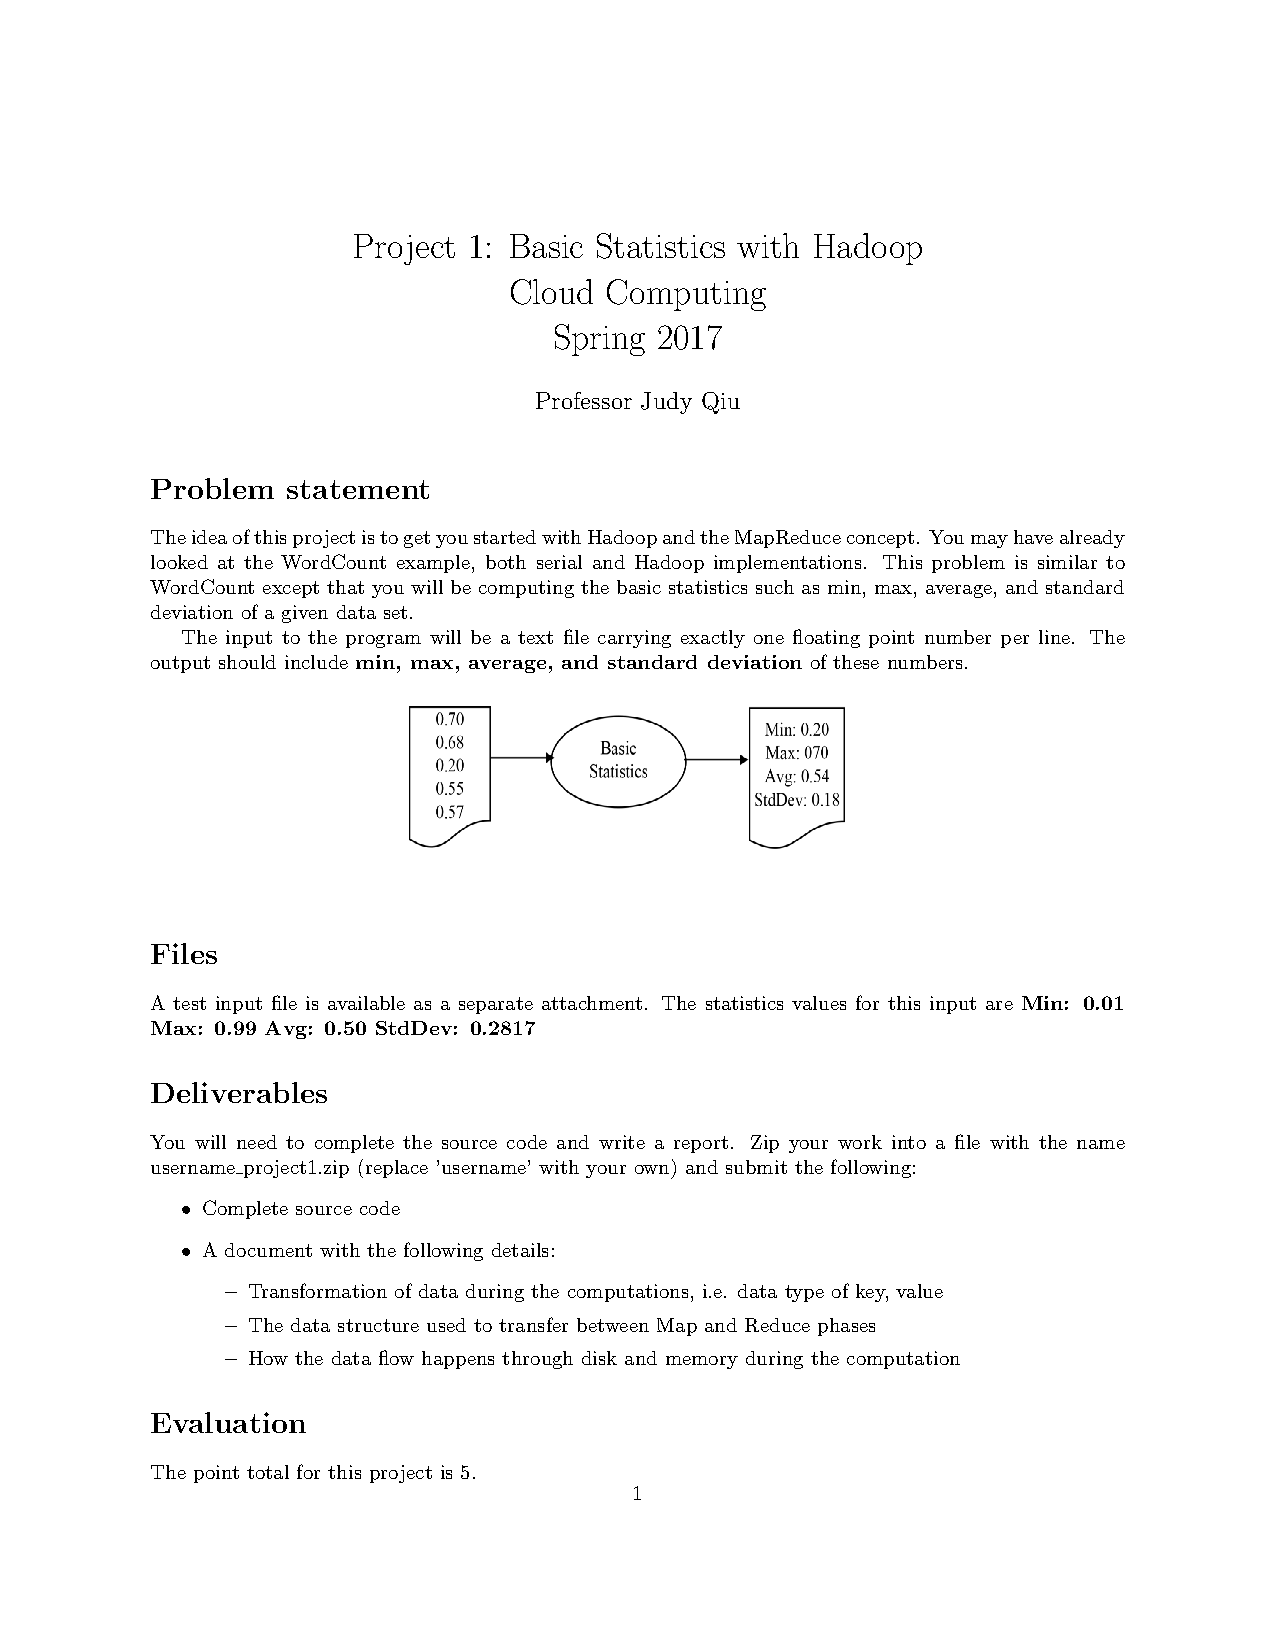
\includepdf[pages=-,pagecommand={},width=\textwidth]{section/icloud/assignment/files/project1.pdf}


\section*{Basic Statistics with Hadoop}       

\subsection*{Problem statement}
 
The idea of this project is to get you started with Hadoop and the MapReduce concept. You may have already looked at the WordCount example, both serial and Hadoop implementations. This problem is similar to WordCount except that you will be computing the basic statistics such as min, max, average, and standard deviation of a given data set.

The input to the program will be a text file carrying exactly one floating point number per line. The output should include \textbf{min, max, average, and standard deviation} of these numbers.

\begin{figure}[!htbp]
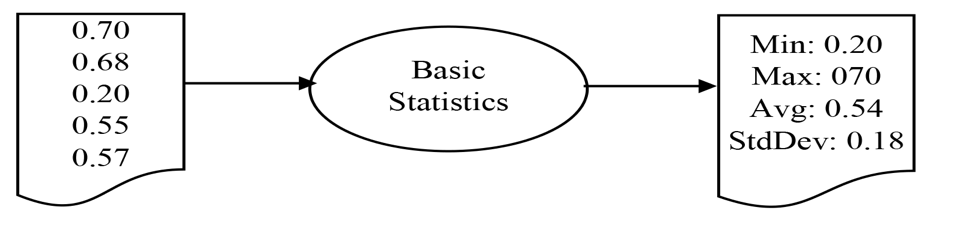
\includegraphics[width=8cm,height=3cm]{section/icloud/assignment/problems/project1/p1example.png}
\centering
\end{figure}

\subsection*{Files}
A test input file is available as a separate attachment.
The statistics values for this input are \textbf{Min: 0.01 Max: 0.99 Avg: 0.50 StdDev: 0.2817}


\subsection*{Deliverables}

You will need to complete the source code and write a report. Zip your work into a file with the name username\_project1.zip (replace 'username' with your own) and submit the following:

\begin{itemize}
\item Complete source code
\item A document with the following details:

  \begin{itemize}
  \item	Transformation of data during the computations, i.e. data type of key, value
  \item	The data structure used to transfer between Map and Reduce phases
  \item	How the data flow happens through disk and memory during the computation
  \end{itemize}

\end{itemize}

\subsection*{Evaluation}

The point total for this project is 5.

\begin{itemize}
\item Correctness of the source code (2 points)
\item	Completeness of the report (3 points)
\end{itemize}



\chapter{Project 2}\label{project-2}

\documentclass{article}
\newtheorem{thm}{Theorem}
\setlength{\oddsidemargin}{0.25in}
\setlength{\textwidth}{6in}
\setlength{\topmargin}{-0.25in}
\setlength{\headheight}{0.3in}
\setlength{\headsep}{0.2in}
\setlength{\textheight}{9in}
\setlength{\footskip}{0.1in}
\usepackage{multirow}
\usepackage{fullpage}
\usepackage{graphicx}
\usepackage{amsthm}
\usepackage{amssymb}
\usepackage{url}
\usepackage{amsfonts}
\usepackage{algpseudocode}
\usepackage{listings}
\usepackage{mathtools}

\usepackage{listings}
\usepackage{color}
 
\definecolor{codegreen}{rgb}{0,0.6,0}
\definecolor{codegray}{rgb}{0.5,0.5,0.5}
\definecolor{codepurple}{rgb}{0.58,0,0.82}
\definecolor{backcolour}{rgb}{0.95,0.95,0.92}
 
\lstdefinestyle{mystyle}{
    backgroundcolor=\color{backcolour},   
    commentstyle=\color{codegreen},
    keywordstyle=\color{magenta},
    numberstyle=\tiny\color{codegray},
    stringstyle=\color{codepurple},
    basicstyle=\footnotesize,
    breakatwhitespace=false,         
    breaklines=true,                 
    captionpos=b,                    
    keepspaces=true,                 
    numbers=left,                    
    numbersep=5pt,                  
    showspaces=false,                
    showstringspaces=false,
    showtabs=false,                  
    tabsize=2
}
 
\lstset{style=mystyle}


\begin{document}\title{Project 2: Hadoop PageRank\\ Cloud Computing\\ Spring 2017}         % Enter your title between curly braces
\author{Professor Judy Qiu }        % Enter your name between curly braces
\date{}          % Enter your date or \today between curly braces
\maketitle
\makeatother     % `@' is restored as a "non-letter" character
\pagestyle{plain}
\section*{Goal}
 
This assignment provides an illustration of PageRank algorithms and Hadoop. You will then blend these applications by implementing a parallel version of PageRank using the programming interfaces of the Hadoop MapReduce framework. 


\section*{Deliverables}
You are required to turn in the following items in a zip file (username\_HadoopPageRank.zip) in this assignment: 
\begin{itemize}
\item The source code of Hadoop PageRank you implemented.
\item Technical report (username\_HadoopPageRank\_report.docx) that contains: 
\item The description of the main steps and data flow in your program. 
\item The output file (username\_HadoopPageRank\_output.txt) which contains the first 10 urls along with their ranks. 
\end{itemize}

\section*{Evaluation}
The point total for this project is 10, where the distribution is as follows:
\begin{itemize}
\item Completeness of your code and output (7 points)
\item Correctness of written report (3 points)
\end{itemize}

\section{What is PageRank?}
The web search engine is a typical distributed system on the Internet. It is designed to search for information on the World Wide Web. The search results are generally presented in a list of results and are often called hits. PageRank is a well-known web graph ranking algorithm that helps Internet users sort hits by their importance. 

PageRank calculates a numerical value for each element of a hyperlinked set of webpages, which reflects the probability that a random surfer will access that page. The process of PageRank can be understood as a Markov Chain which requires iterative calculations to converge. An iteration of PageRank calculates the new access probability for each webpage based on values calculated in the previous iteration. The process will repeat until the number of current iterations is bigger than predefined maximum iterations, or the Euclidian distance between rank values in two subsequent iterations is less than a predefined threshold that controls the accuracy of the output results. 

\begin{figure}[!htbp]
\centering
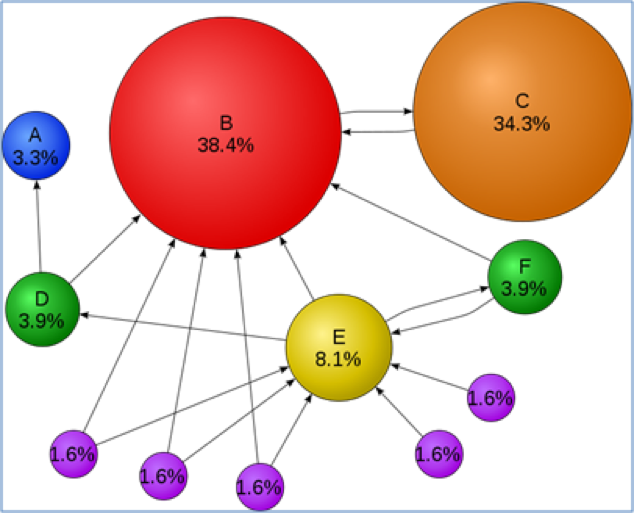
\includegraphics[width=8cm]{pagerankexample}
\caption{Mathematical PageRank for a simple network in Wikipedia}
\label{fig:pagerankexample}
\end{figure}

Figure~\ref{fig:pagerankexample} shows a web graph consisting of 11 vertices {A, B, C, D, E, F, G1, G2, G3, G4, G5}. Each vertex refers to a unique webpage, and the directed edge means there is one link from the source webpage to the target webpage. The percentage on each vertex represents the rank value of each webpage.

\subsection*{Notes}

You can implement a sequential PageRank that can run on desktops or laptops. But when processing larger input data, like web graphs containing more than a million webpages, you need to run the PageRank application in parallel so that it can aggregate the computing power of multiple compute nodes. Currently, in both industry and academia, the study of large-scale web or social graphs has become increasingly popular. In one published paper, the job execution engines that claim to support large-scale PageRank include: MPI, Hadoop, Dryad, Twister, Pregel. 

\subsection*{Formula}

Equation~\ref{eq:pagerank} is the formula to calculate the rank value for each webpage. We will learn this formula by applying it to the case in Figure~\ref{fig:pagerankexample}. There are 11 webpages in Figure~\ref{fig:pagerankexample}, which include: {A, B, C, D, E, F, G1, G2, G3, G4, G5}. Assuming the probability distribution for a web surfer accessing all these 11 pages in current iteration is \{PR(A), PR(B), PR(C), ... PR(G5)\}, then the probability for the surfer to access Page B in the next iteration is: \\

$PR(B) = PR(D)/2 + PR(E)/3 + PR(F)/2 + PR(C) + PR(G1)/2 + PR(G2)/2 + PR(G3)/2 $\\


In a general case, the PageRank value for any page u can be expressed as:

\begin{equation}\label{eq:pagerank}
PR(u) = \sum_{v \in Set} \frac{PR(V)}{L(v)}
\end{equation}

The vertices seen in the right of the formula contain all the webpages that point to target webpage 'u'. The L(v) refers to the out degree of each webpage in the vertices set. The initial rank values of each webpage, like PR'(u), can be any double value. After several iteration calculations, the rank values converge to the stationary distribution regardless of what their initial values are.

\subsection*{Damping factor}
The PageRank theory holds that even an imaginary surfer who is randomly clicking on links will eventually stop clicking. The probability, at any step, that the person will continue is a damping factor d. Various studies have tested different damping factors, but it is generally assumed that the damping factor will be around 0.85. The formula considering damping factor is shown in Equation~\ref{eq:pagerankwithdf}. N refers to the total number of unique urls. 

\begin{equation}\label{eq:pagerankwithdf}
PR(u) = \frac{1-d}{N} + d * \sum_{v \in Set} \frac{PR(V)}{L(v)}
\end{equation}

\section*{Hadoop PageRank DataFlow}
In this project, we have provided a sketch code which contains three MapReduce jobs for you to implement:
\begin{itemize}
\item CreateGraph (done): add one column, 'initial pagerank value', to the input pagerank adjacency matrix (AM). Then pass it to the PageRank program to calculate the pagerank values. 
\item PageRank (your implementation): take the transformed AM matrix and calculate pagerank values for all pages. 
\item Cleanup Results: remove the targetUrls column and output \textbf{(sourceUrl, pagerank value)} as the final result. 
\end{itemize}

The detail dataflow can be seen in Figure~\ref{fig:hadoopdataflow}. Part 1 and Part 3 are given as full solutions in this pipeline; you will implement the 2nd part of the PageRank program.
\begin{figure}[!htbp]
\centering

\includegraphics[width=10cm]{hadoopdataflow.png}
\caption{Hadoop PageRank dataflow}
\label{fig:hadoopdataflow}
\end{figure}

Normally for any Hadoop MapReduce program, input data is uploaded and stored in the Hadoop Distributed File System (HDFS) before computation in order to generate \textbf{(key, value)} pairs to the mapper. Initially, the PageRank input data is stored in the format of adjacency matrix as a file(s) in the local file system. Then it will be uploaded to the HDFS and distributed across the compute nodes. Hadoop framework reads the application records from HDFS with the InputFormat interface and generates \textbf{(key, value)} pair input streams. Each Map function produces zero or more intermediate \textbf{(key, value)} pairs by consuming one input (key, value) pair. For this PageRank program, the map function applies the calculation $\frac{PR(v)}{L(V)}$ to each \textbf{(key, value)} pair, where the key is the unique id or name of the webpage and the value contains the current rank value of the webpage and its out link information. Map tasks then generate intermediate (key, value) pairs, whose value is the partial rank value of every webpage. Each reduce task aggregates all the partial values of specific webpages by applying the provided Equation~\ref{eq:pagerankwithdf}. The aggregated global rank values are written back to HDFS, which in turn is used as input in the next set of iterations, if any. "Hadoop - PageRank" in Figure~\ref{fig:hadoopdataflow} shows an example for the PageRank data processing.


\section*{Code for Hadoop PageRank}

You need to complete two files in the provided pacakge inside "indiana/cgl/hadoop/pagerank/": PageRankMap.java and PageRankReduce.java. Code snapshots are shown below.

\lstinputlisting[language=Java]{PageRankMap.java}
\lstinputlisting[language=Java]{PageRankReducer.java}

\section*{Edit}
The sketch code is stored within the provided VirtualBox image. Use Eclipse or linux text editor vi/vim to add your code.
\begin{lstlisting}[language=bash]
$ cd /root/MoocHomeworks/HadoopPageRank/
$ vim src/indiana/cgl/hadoop/pagerank/PageRankMap.java
$ vim src/indiana/cgl/hadoop/pagerank/PageRankReduce.java
\end{lstlisting}

\section*{Compile and run your code}
Use the one-click script compileAndExecHadoopPageRank.sh provided below. Standard error messages such as compile errors, execution errors, etc. will be redirected on the screen. Debug them based on the returned messages.
\begin{lstlisting}[language=bash]
$ cd /root/MoocHomeworks/HadoopPageRank/
# usage: ./compileAndExecHadoopPageRank.sh [PageRank Input File][Number of Urls][Number Of Iterations]
$ ./compileAndExecHadoopPageRank.sh PageRankDataGenerator/pagerank5000g50.input.0 5000 1
\end{lstlisting}

\section*{View the result}
The result is generated as /root/hbaseMoocAntProject/output/project2.txt. 
\begin{lstlisting}[language=bash]
$ cd /root/MoocHomeworks/HadoopPageRank/
$ cat output/*
\end{lstlisting}


\bibliographystyle{unsrt} 
\end{document}


You are required to turn in the following items in a zip file
(username\_HadoopPageRank.zip) in this assignment:

\begin{itemize}
\item
  The source code of Hadoop PageRank you implemented.
\item
  \begin{description}
  \item[Technical report (username\_HadoopPageRank\_report.docx) that
  contains:]
  \begin{itemize}
  \tightlist
  \item
    The description of the main steps and data flow in your program.
  \item
    The output file (username\_HadoopPageRank\_output.txt) which
    contains the first 10 urls along with their ranks.
  \end{itemize}
  \end{description}
\end{itemize}

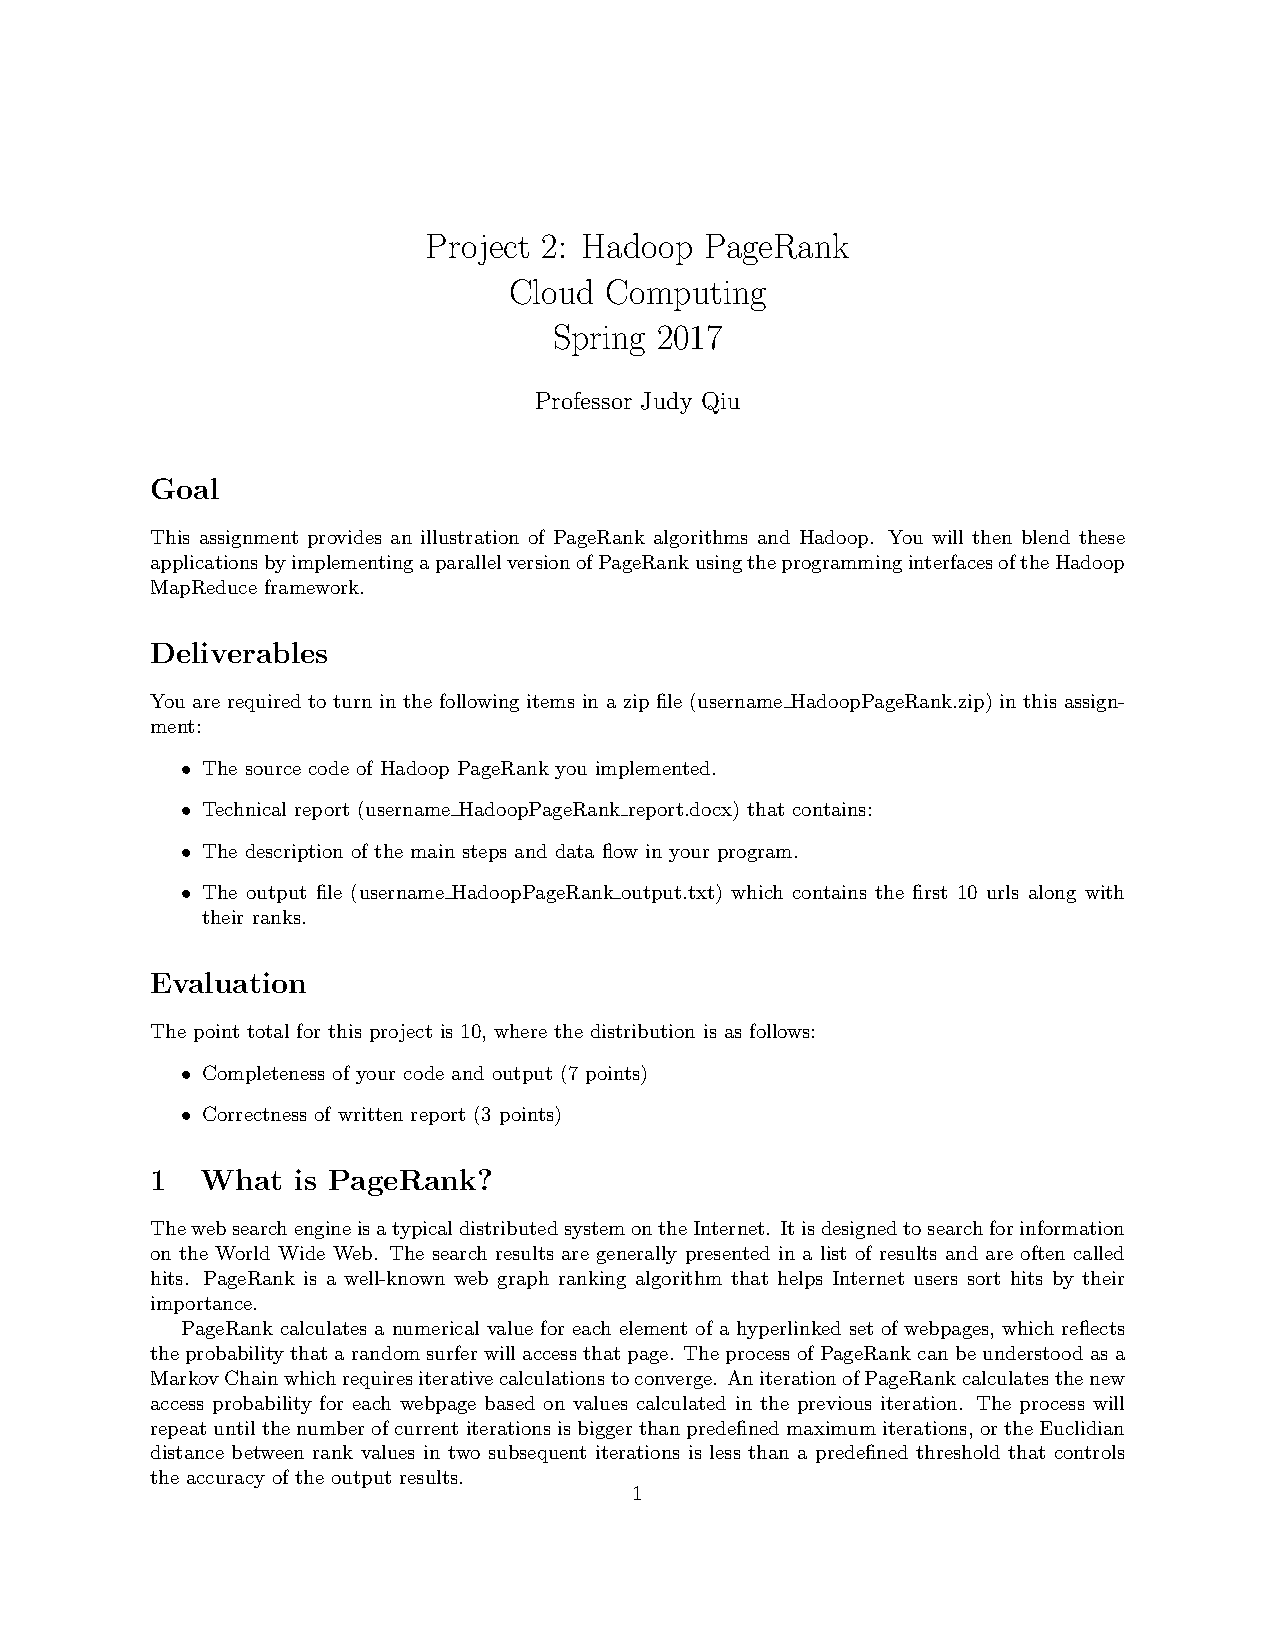
\includepdf[pages=-,pagecommand={},width=\textwidth]{section/icloud/assignment/files/project2.pdf}

\chapter{Project 3}\label{project-3}

Project 3 asks you to implement a bioinformatics application using
Hadoop (Map only) MapReduce framework and write a report about the data
flow and your observations of the program.

You are required to turn in the following items in a zip file
(username\_HadoopBlast.zip) in this assignment:

\begin{itemize}
\tightlist
\item
  The source code of Hadoop Blast you implemented.
\item
  Technical report (username \_HadoopBlast\_report.docx) that answers
  the following questions. - What is Hadoop Distributed Cache and how is
  it used in this program? - Write the two lines that put and get values
  from Distributed cache. Also include the method and class information.
  - In previous projects we used Hadoop's TextInputFormat to feed in the
  file splits line by line to map tasks. In this program, however, we
  want to feed in a whole file to a single map task. What is the
  technique used to achieve this? Also, briefly explain what are the key
  and value pairs you receive as input to a map task and what methods
  are responsible for producing these pairs? - Do you think this
  particular implementation will work if the input files are larger than
  the default HDFS block size? Briefly explain why. [Hint: you can
  test what will happen by concatenating the same input file multiple
  times to create a larger input file in the resources/blast\_input
  folder] - If you wanted to extend this program such that all output
  files will be concatenated into a single file, what key and value
  pairs would you need to emit from the map task? Also, how would you
  use these in the reduce that you would need to add?
\item
  The 4 output FASTA files -- celllines\_1.fa to celllines\_4.fa.
\end{itemize}

Points will be reduced (maximum 0.5 points) if the filename or directory
structure are different from instructed above.

The point total for this project is 3, where the distribution is as
follows:

\begin{itemize}
\tightlist
\item
  Completeness of your code and output (1 points)
\item
  Correctness of written report (2 points)
\end{itemize}

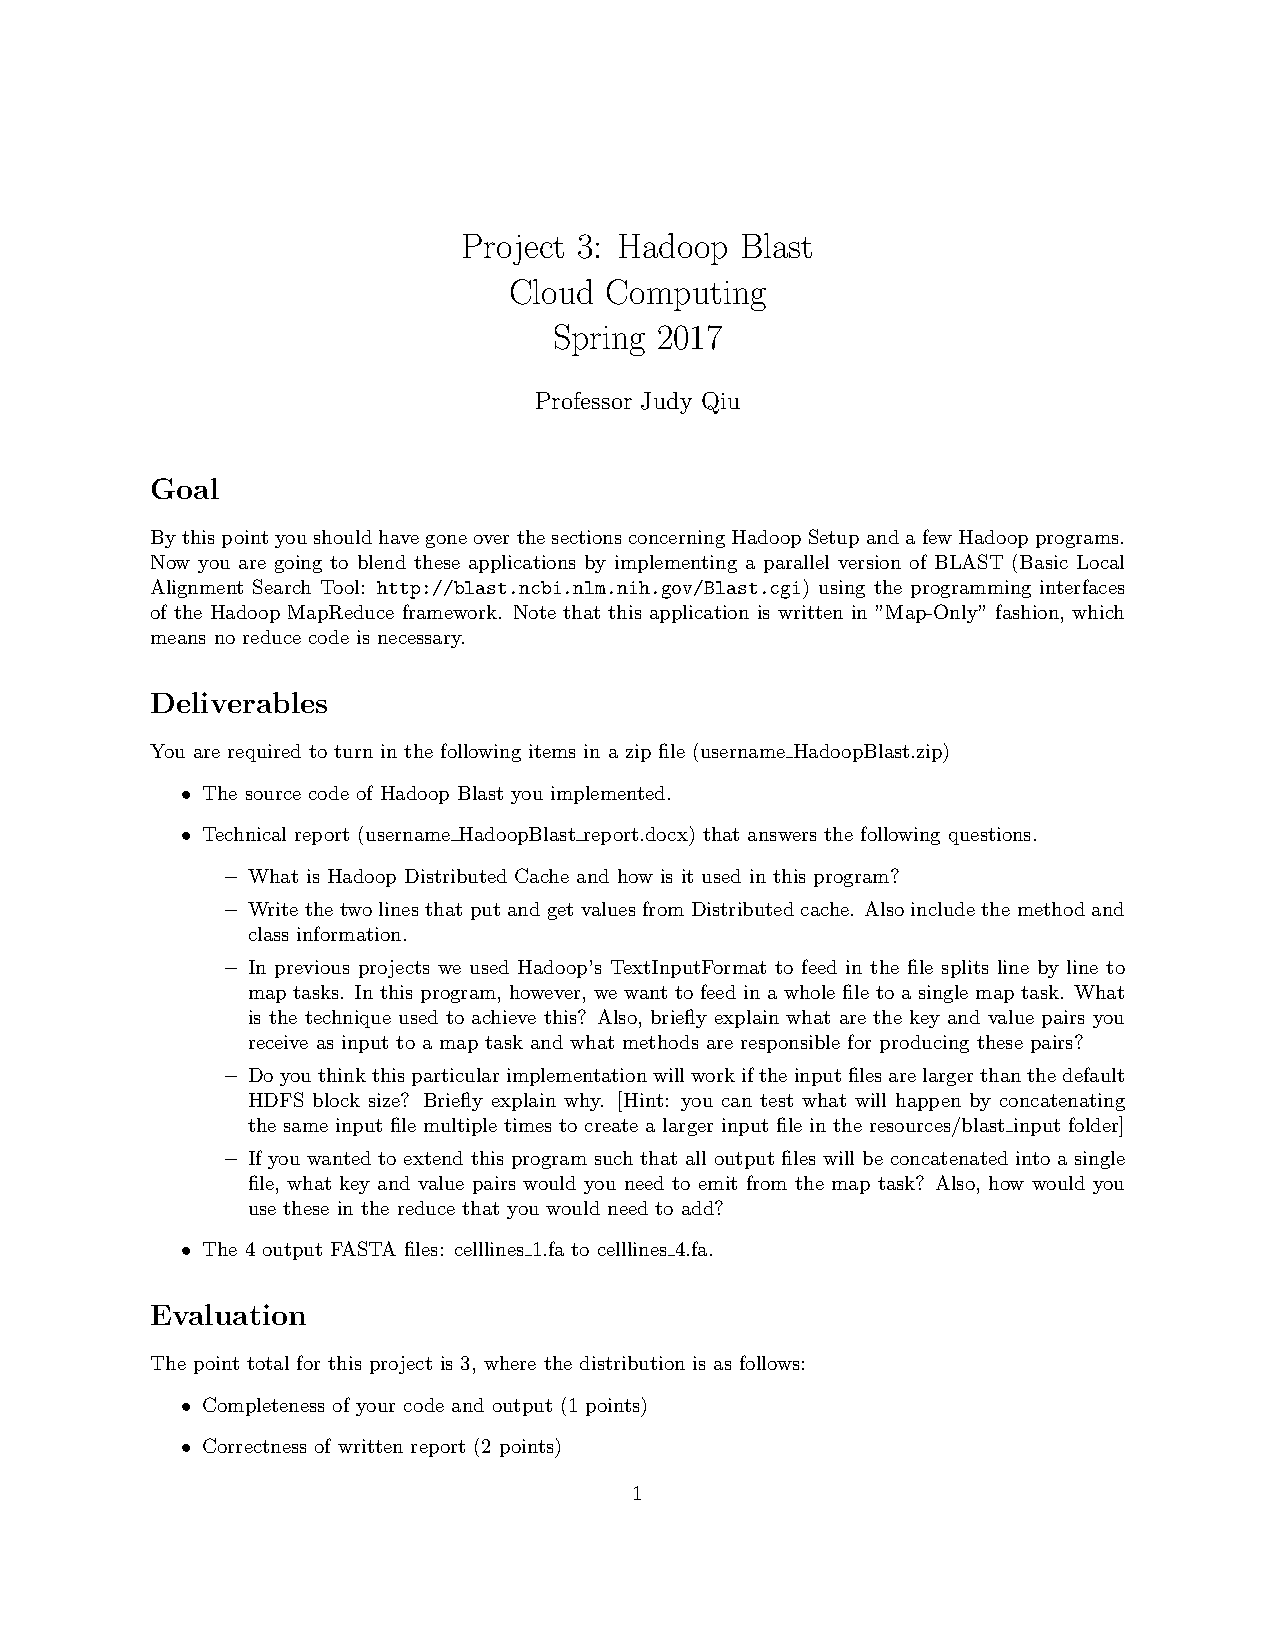
\includepdf[pages=-,pagecommand={},width=\textwidth]{section/icloud/assignment/files/project3.pdf}

\chapter{Project 4}\label{project-4}

Zip your source code and report in a file named username\_project4.zip

The point total for this project is 1.5, where the distribution is as
follows:

\begin{itemize}
\tightlist
\item
  Correctness of your code and output (1 points)
\item
  Completeness of written report (0.5 points)
\end{itemize}

Before you start this project, you need to complete the
Project4 Prerequisite\textless{}files/project4\_pre.pdf\textgreater{}
first. The submission folder for it will be published before the lab
session.

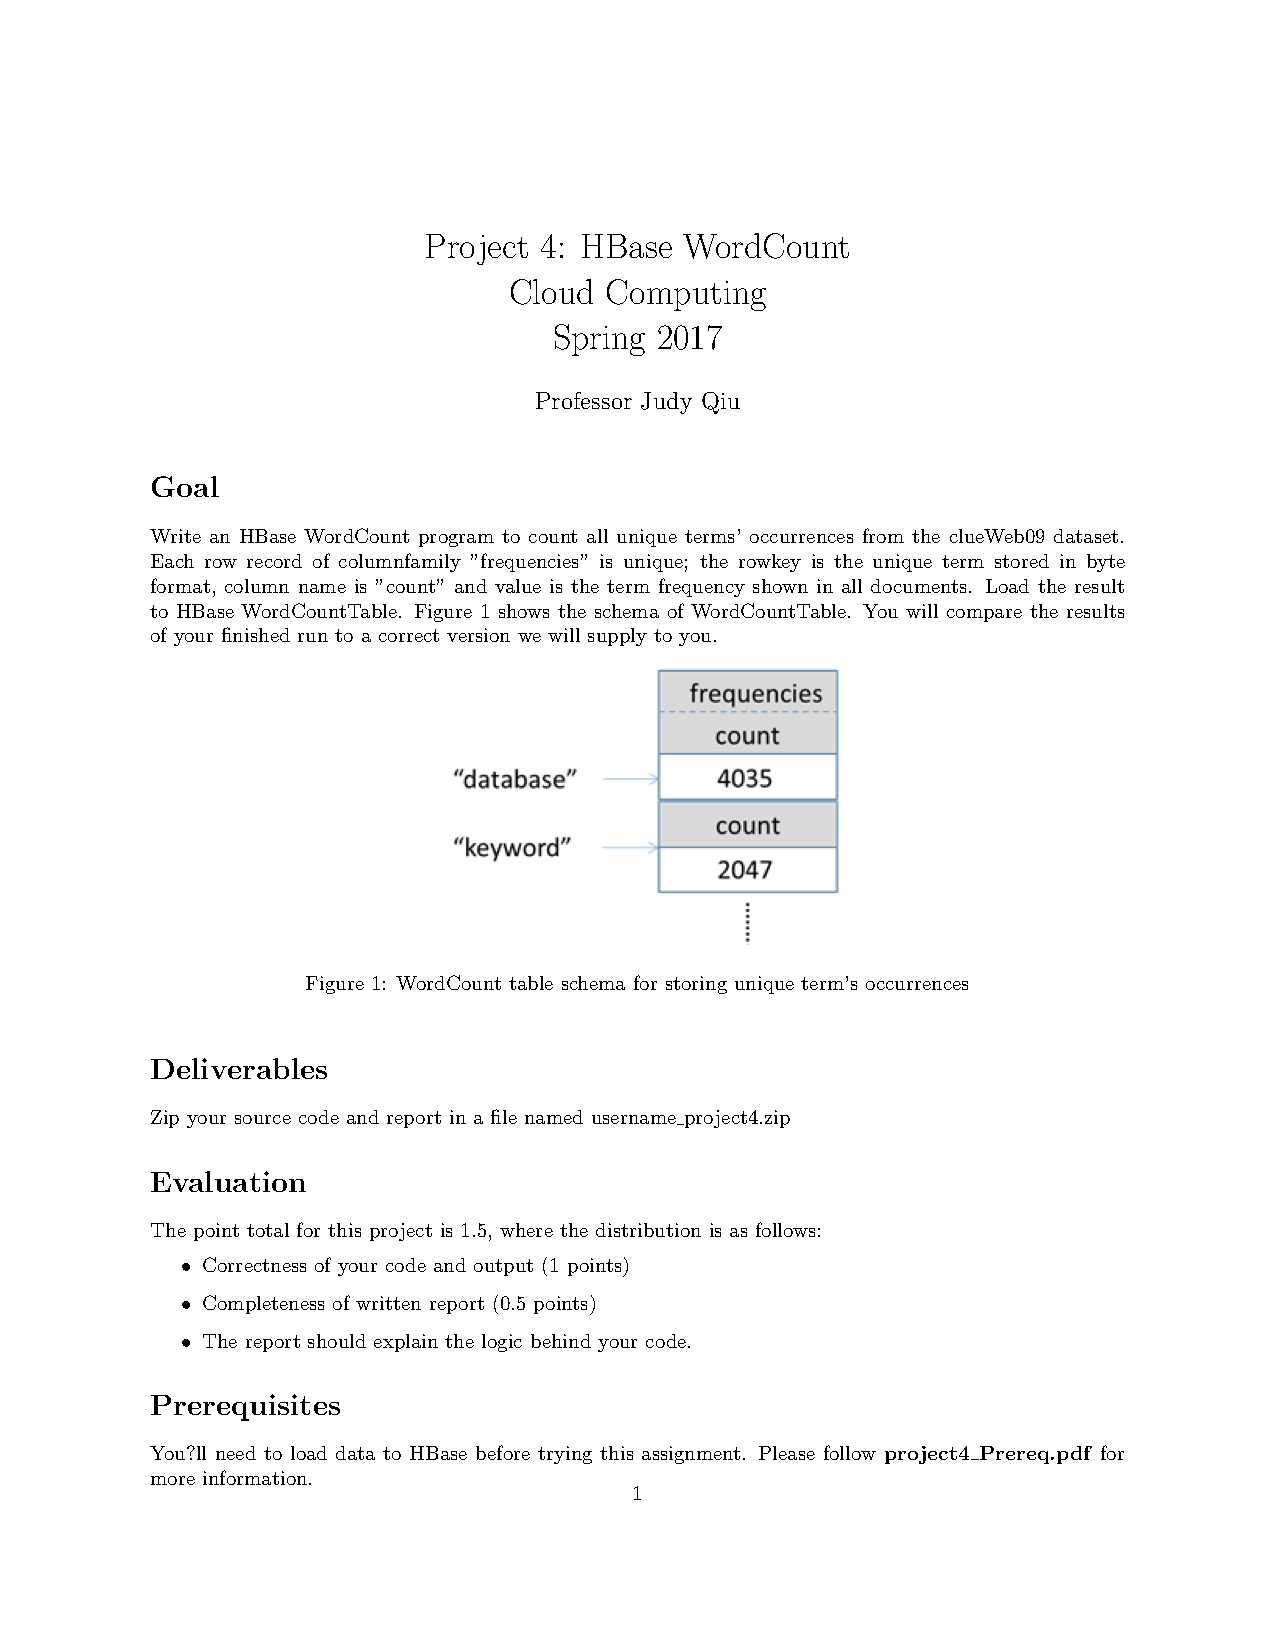
\includepdf[pages=-,pagecommand={},width=\textwidth]{section/icloud/assignment/files/project4.pdf}
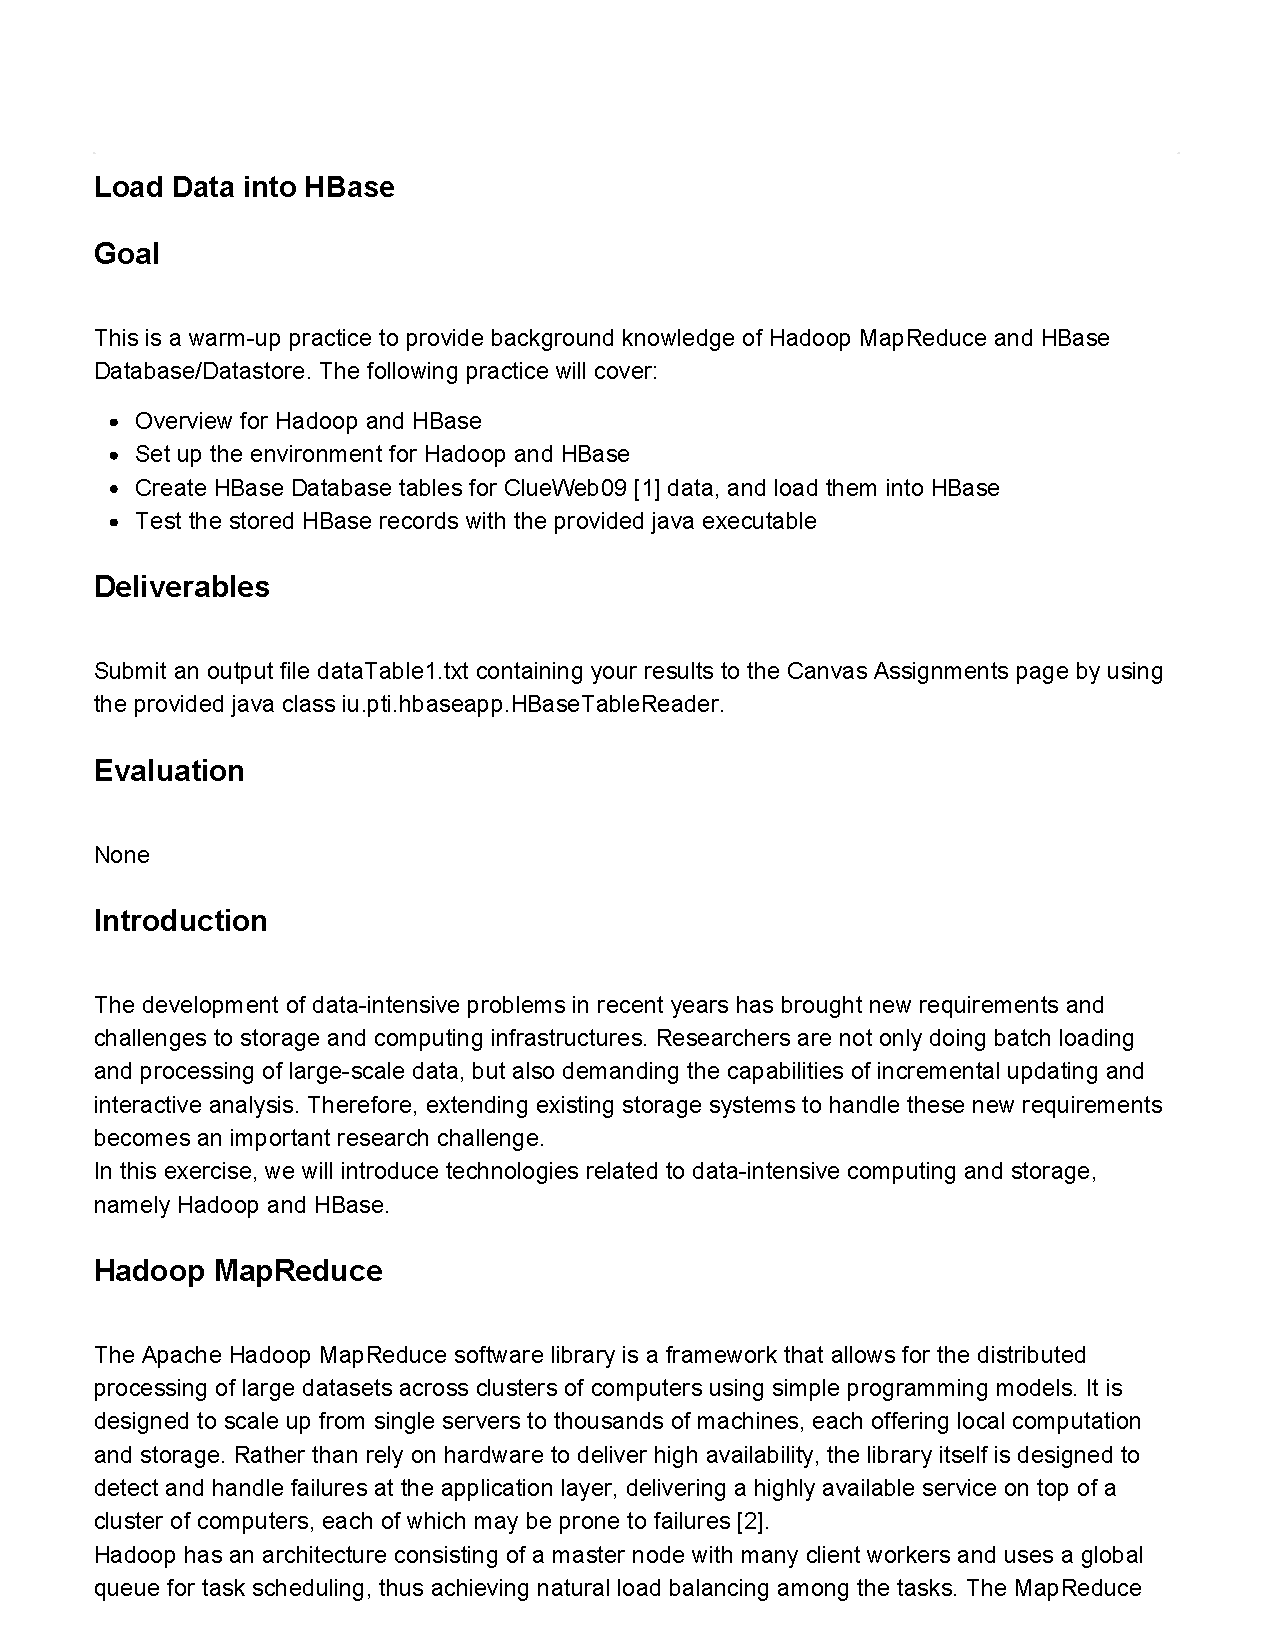
\includepdf[pages=-,pagecommand={},width=\textwidth]{section/icloud/assignment/files/project4_pre.pdf}

\chapter{Project 5}\label{project-5}

Write an HBase FreqIndexBuilder program to build an inverted index table
which has the unique term's occurrences in all documents from the
clueWeb09 dataset. Zip your source code, results and report in a file
named username\_project5.zip. Submit this file to the Canvas submission
page.

\begin{itemize}
\tightlist
\item
  Complete source code
\item
  A written report describing the main steps
\end{itemize}

The point total for this project is 3, where the distribution is as
follows:

\begin{itemize}
\tightlist
\item
  Completeness of your code and output (2 points)
\item
  Correctness of written report (1 points)
\end{itemize}

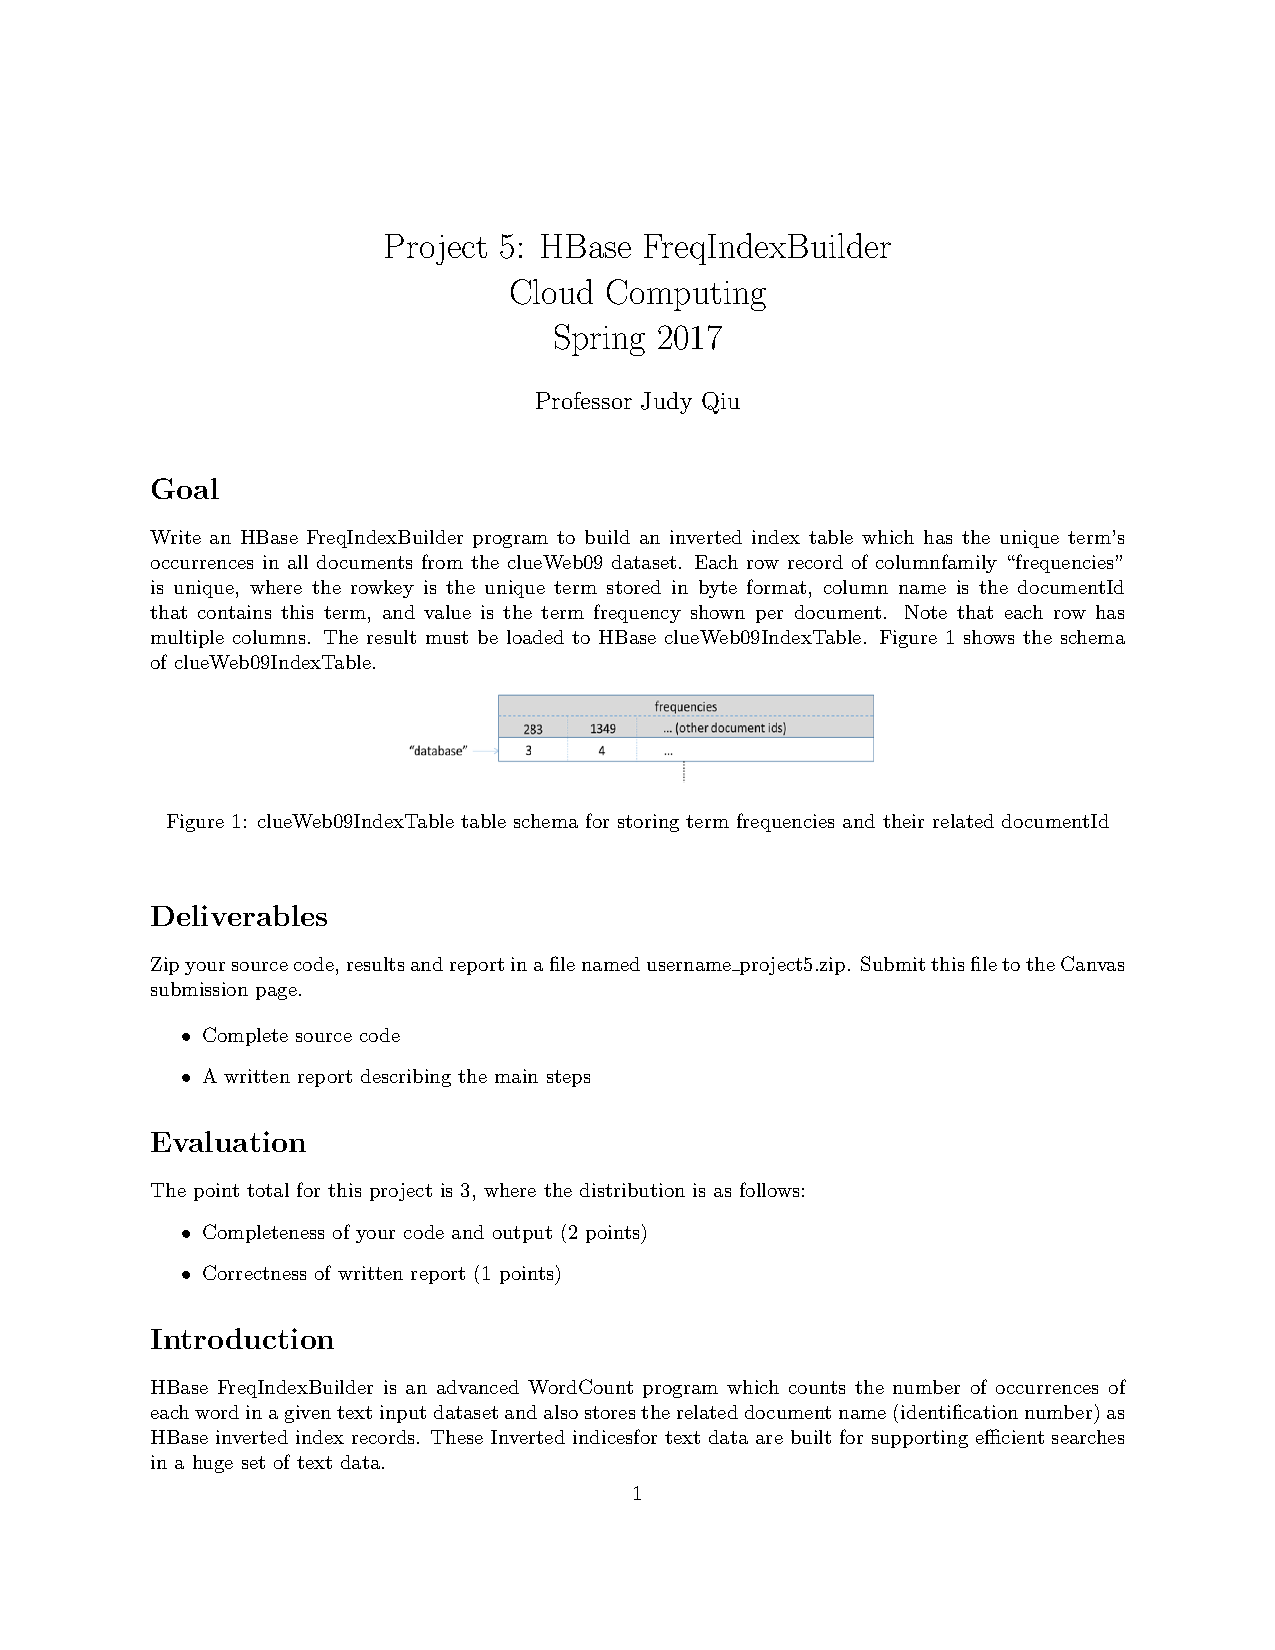
\includepdf[pages=-,pagecommand={},width=\textwidth]{section/icloud/assignment/files/project5.pdf}

\chapter{Project 6}\label{project-6}

After having familiarized yourself with the ``HBase Building an Inverted
Index'' homework and ``PageRank algorithms'' homework, you are ready to
use these applications to test the search engine function from the
packaged executable.

\section{Deliverables}\label{deliverables}

Zip your source code, library, and results in a file named
\href{mailto:username@test-search-engine.zip}{\nolinkurl{username@test-search-engine.zip}}.
Please submit this file to the Canvas Assignments page.

\section{Evaluation}\label{evaluation}

The point total for this project is 6, where the distribution is as
follows:

\begin{itemize}
\tightlist
\item
  Completeness of your code (5 points)
\item
  Correct output (1 points)
\end{itemize}

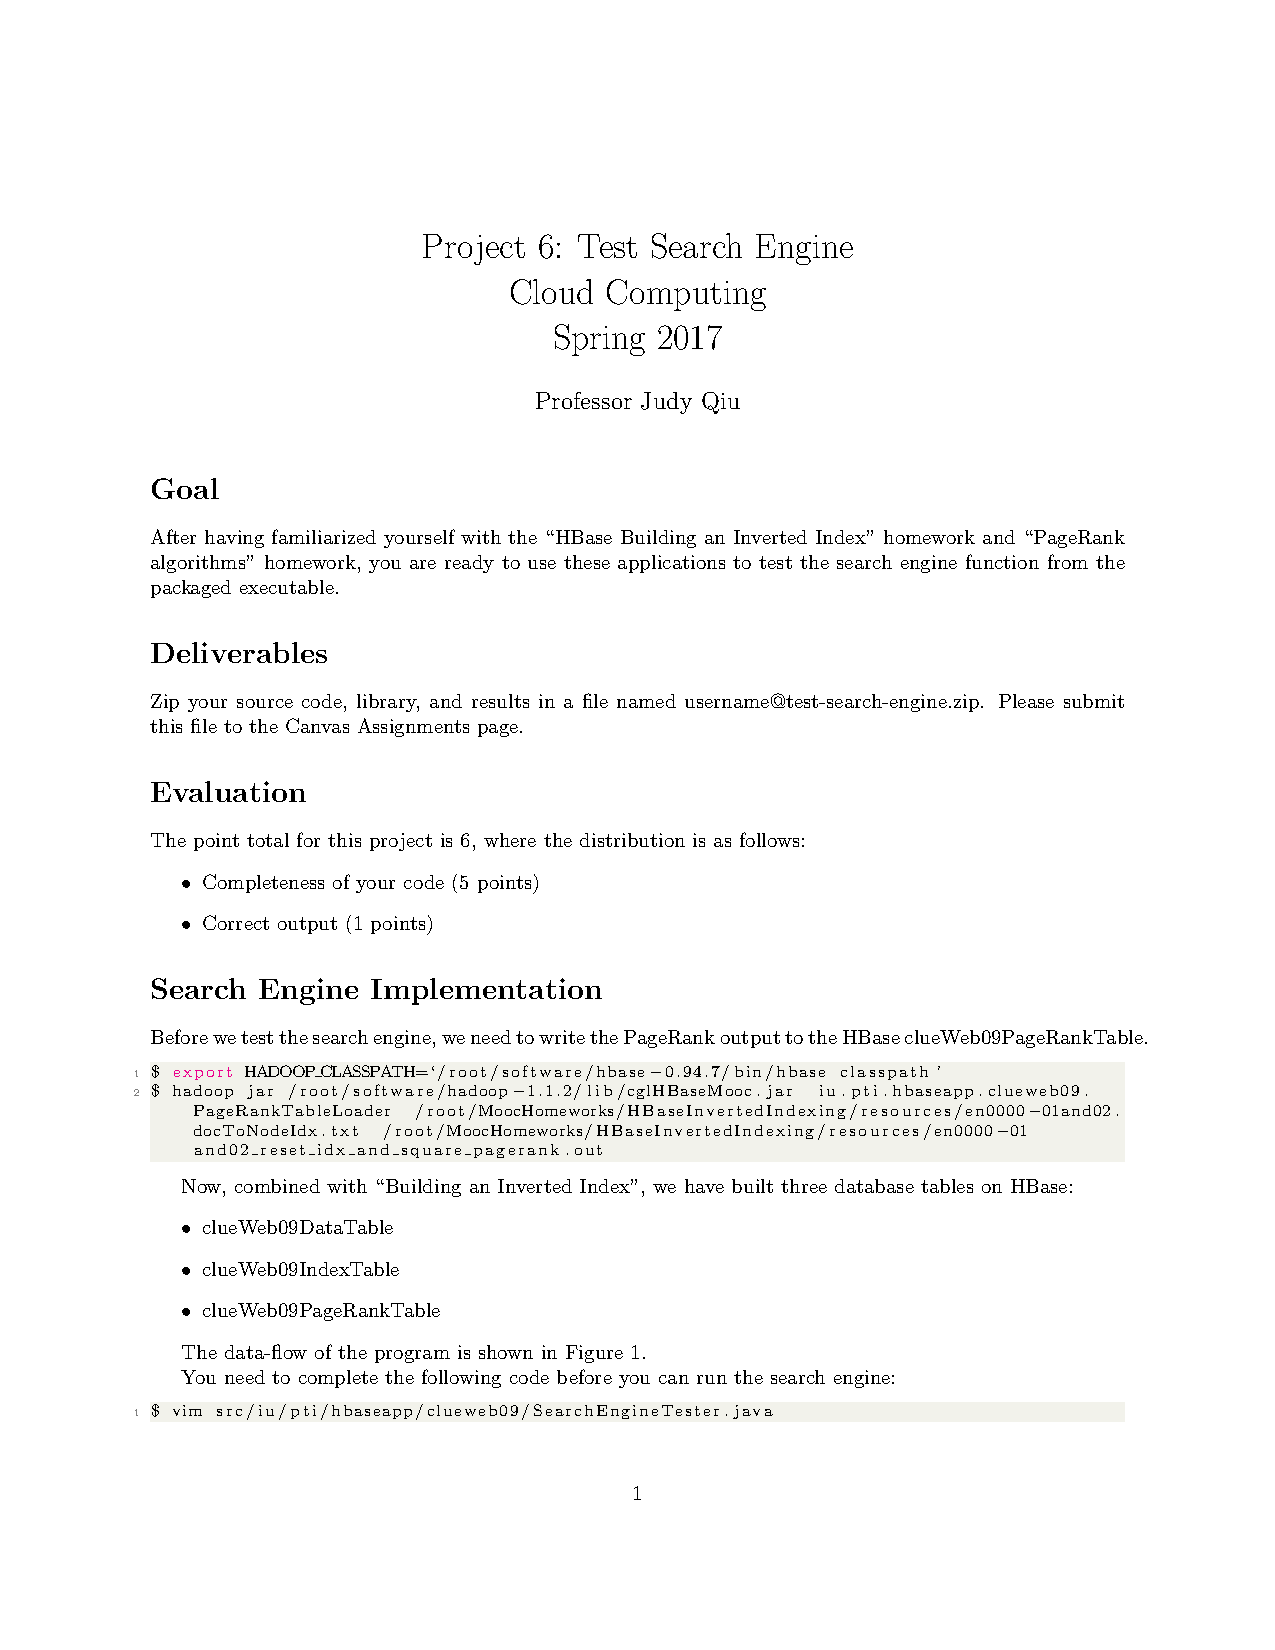
\includepdf[pages=-,pagecommand={},width=\textwidth]{section/icloud/assignment/files/project6.pdf}

\chapter{Project 7}\label{project-7}

The goal of this project is to familiarize yourself with the concept of
map-collective applications. Harp is similar to MapReduce in terms of
programming with the exception that it provides collective communication
support across map tasks.

Zip your source code and output as username\_harp-pagerank.zip. Please
submit this file to the Assignments page.

The point total for this project is 6, where the distribution is as
follows:

\begin{itemize}
\tightlist
\item
  Completeness of your code (5 points)
\item
  Correct output (1 point)
\end{itemize}

We prepared a new VM for project7 and project8. Please download it from
\href{https://drive.google.com/file/d/0B2iFsq4CY1DteHhJUEk5cDNJajQ/view}{here}.

\begin{itemize}
\tightlist
\item
  \href{https://drive.google.com/file/d/0B2iFsq4CY1DteHhJUEk5cDNJajQ/view}{VirtualBox
  VM Download}
\end{itemize}

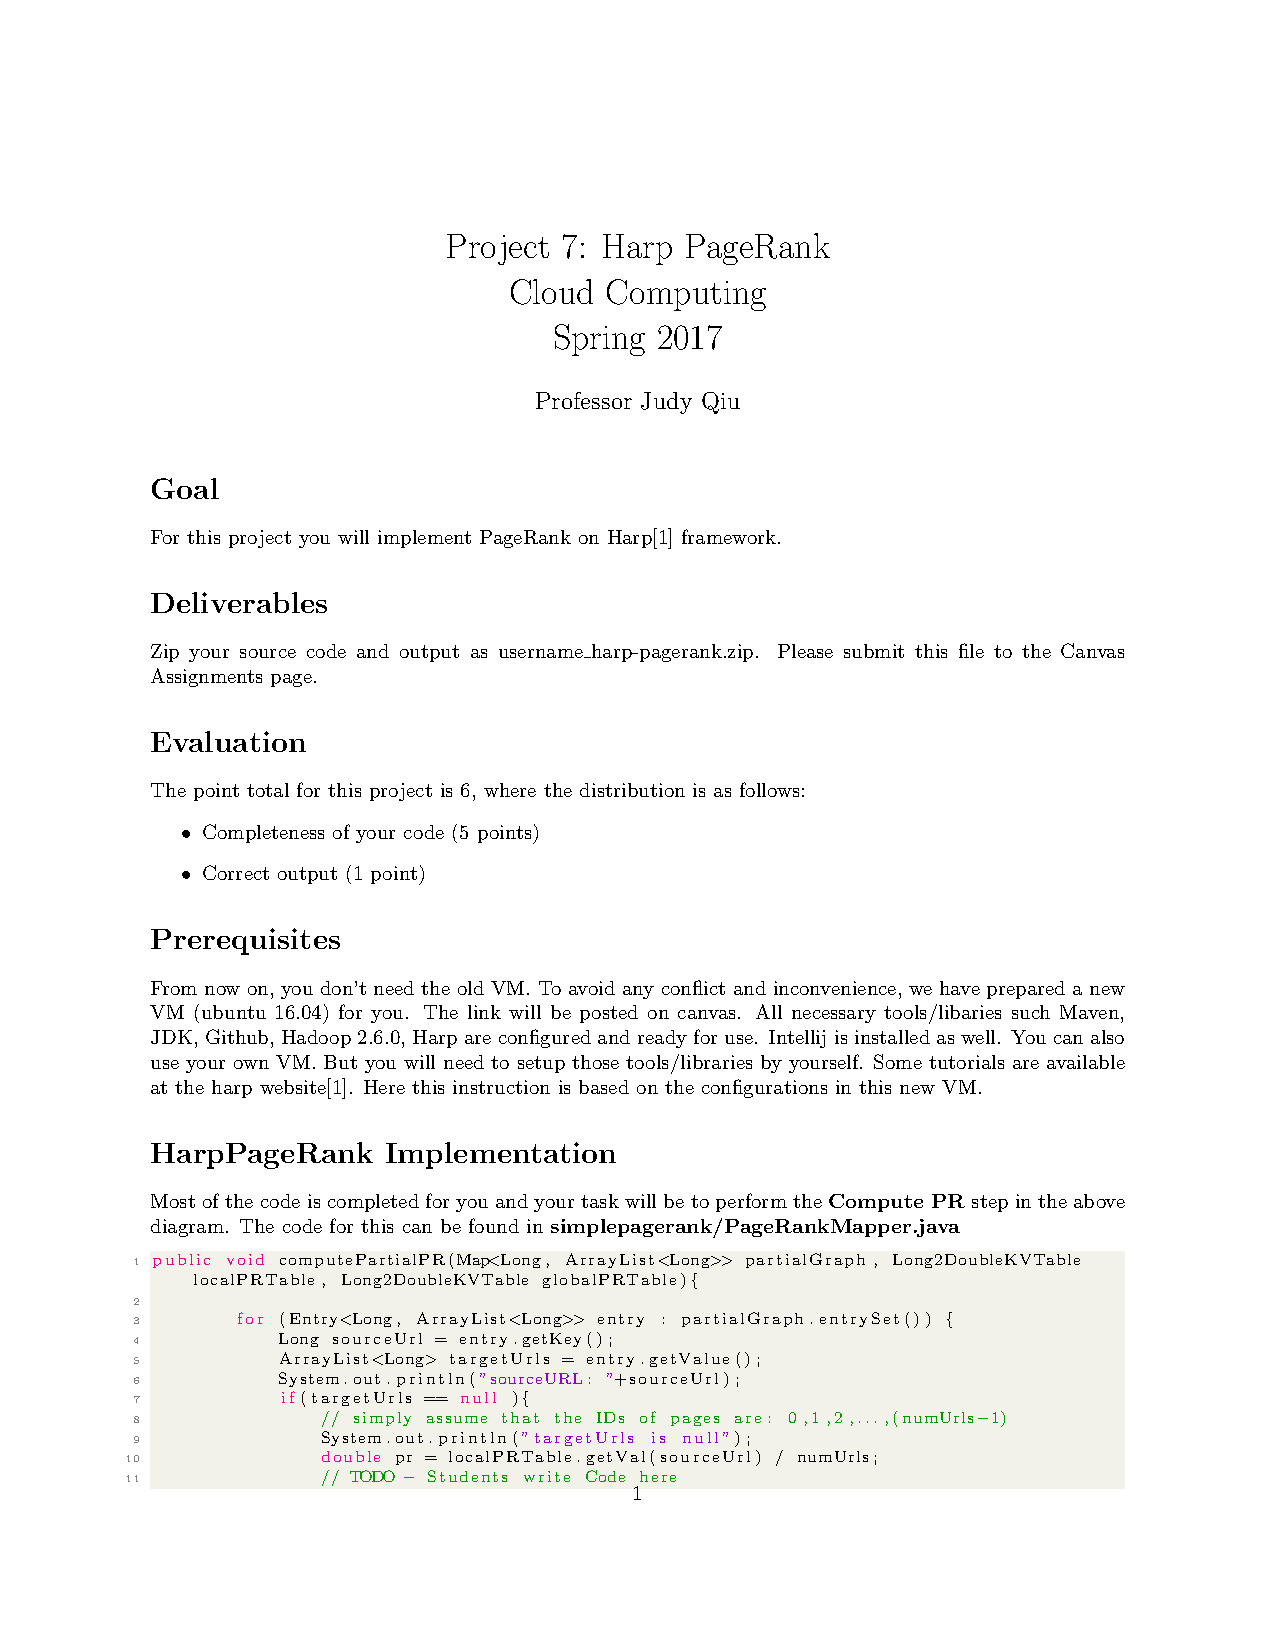
\includepdf[pages=-,pagecommand={},width=\textwidth]{section/icloud/assignment/files/project7.pdf}

\begin{description}
\item[Do not copy and paste commands from pdf files. Please type them]
manually. Special characters cause problems in executing commands in a
terminal.
\end{description}

\chapter{Project 8}\label{project-8}

Zip your source code and report as username\_mbkmeans.zip.

The point total for this project is 6, where the distribution is as
follows: - Completeness of your code (5 points) - In the report,
describe your implementation and the output. (1 points)

You can get up to 4 bonus points based on your extra efforts.

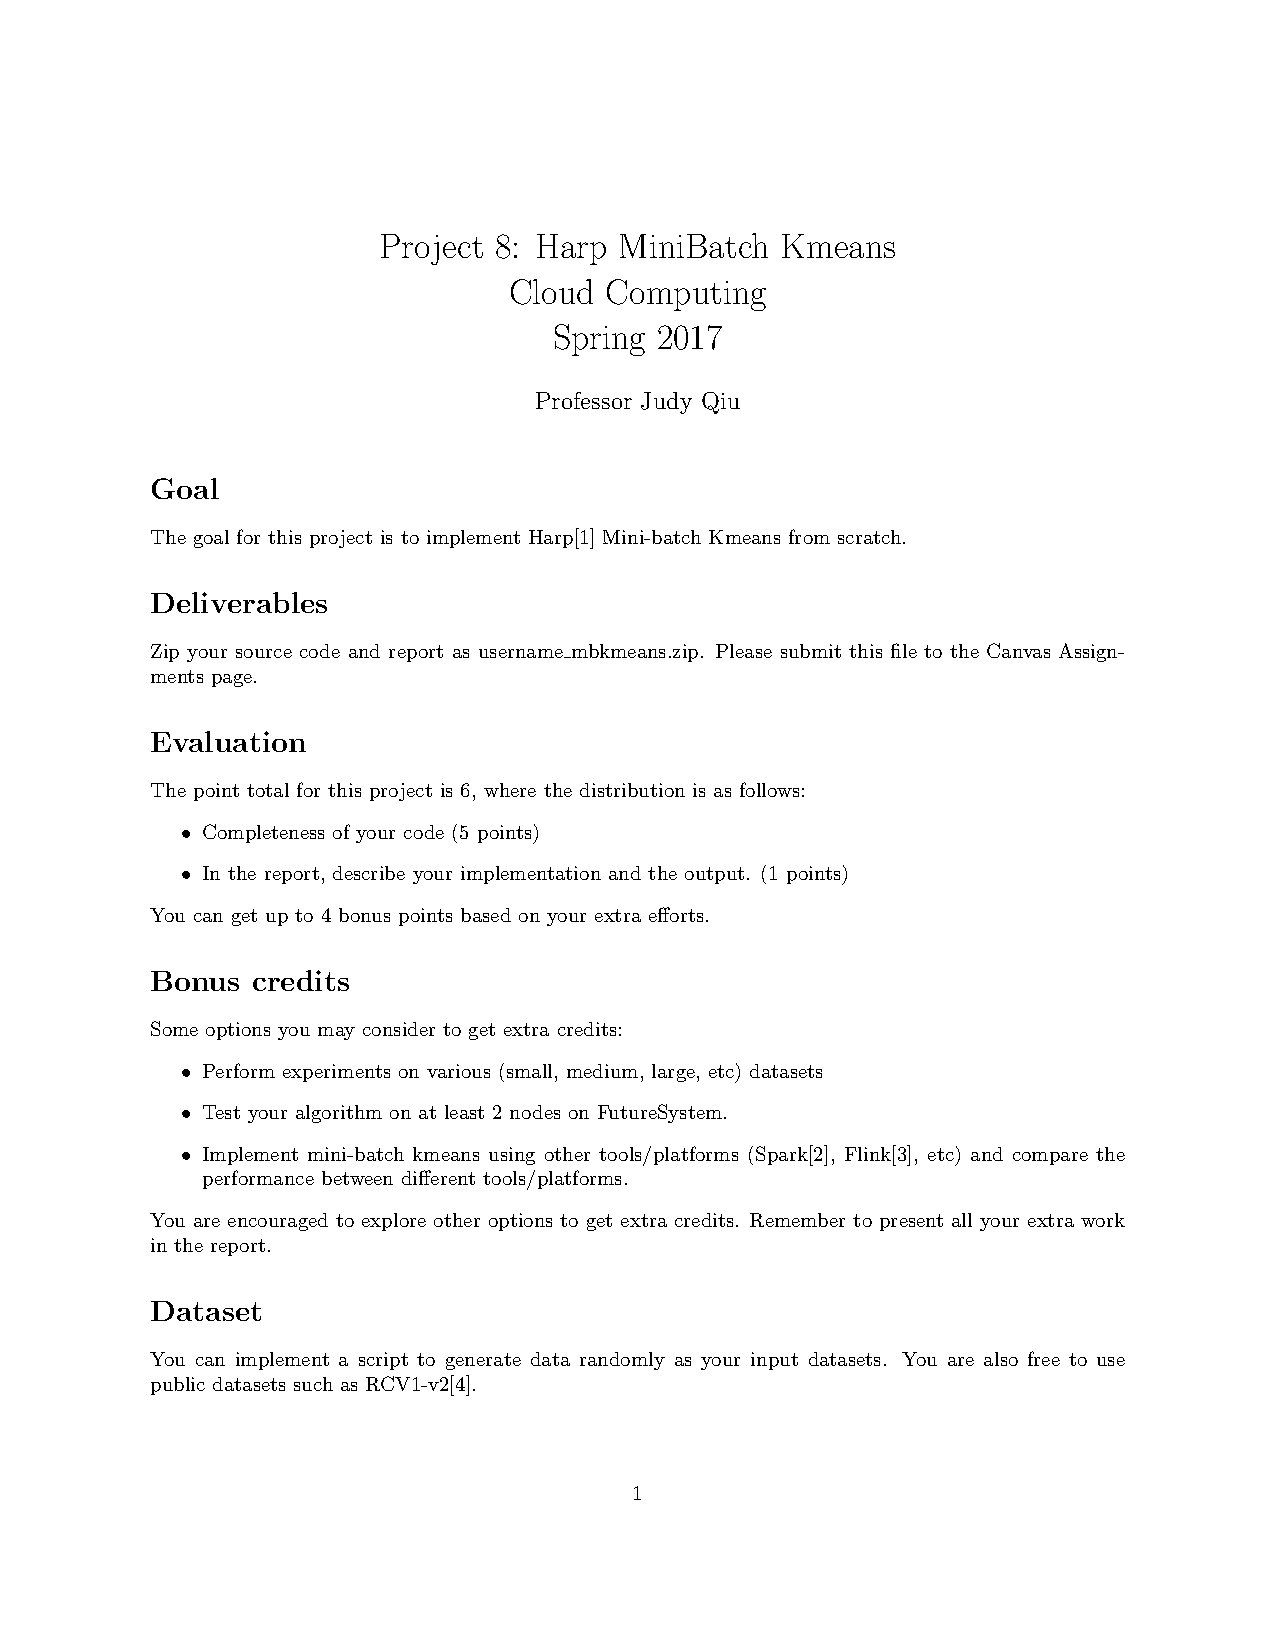
\includepdf[pages=-,pagecommand={},width=\textwidth]{section/icloud/assignment/files/project8.pdf}
